\documentclass{puzzlehunt}
\usetikzlibrary{calc,shapes,patterns,arrows}

\usepackage[puttinydots]{braille}
\usepackage{multicol}
\usepackage{fontenc}
\usepackage{wedn}
\usepackage{tikz}
\usepackage{txfonts}

\phSetTitle{MaPP Challenge '20 -- Mystery of the Missing Archeologist}
\phSetAuthor{Mathematical Puzzle Programs}
% \phUseAuthorWithTitle

%\phMarkDraft % comment out to remove draft watermark
%\phShowPageNumbers % comment out to hide page numbers

% replace these with your image files
\phSetBannerLogo{assets/mapp-banner}
\phSetSquareLogo{assets/mapp-square}

\input{puzzles/custom-commands}

\begin{document}

\phTitlePage % Prints title page.
%\phTableOfContents % Prints table of contents

\phChapterWorksheet{How to Play}{Rules}

  \phSection{Leagues}

Each team is registered in either the \textbf{Competitive or Recreational League}.
If both Leagues are playing simultaneously today at your campus, then all
scoring and awards are handled separately in both Leagues.

\phSection{Puzzle Packets and ClueKeeper}

Each team has received multiple \textbf{Puzzle Packets}. However, there is
not enough information in this packet to begin solving any puzzles.

Once the game begins, clues will become available in the \textbf{ClueKeeper} app that
will allow players to begin solving puzzles in the packet. Once a puzzle is
solved, its solution can be submitted via the app. As time progresses, hints
for unsolved puzzles will unlock, helping teams who are stuck. The game
ends when your time in ClueKeeper has expired.

\phSection{Main Puzzles}

Once the game begins, you'll be presented with four \textbf{Main Puzzles}. 
Each Main Puzzle can be solved directly using mathematical modeling
and problem-solving abilities. Once the solution for the puzzle has been
entered into ClueKeeper, \textbf{1000 Victory Points} will be awarded,
and the second part will be unlocked. This second part uses the first
solution to extract a short word or phrase. Solving this second challenge
is worth an additional \textbf{500 Victory Points}.

\phSection{Cryptic Puzzles}

After solving the second part of each Main Puzzle, an additional
\textbf{Cryptic Puzzle} will become available to solve.
The way to solve these puzzles is left, well,
cryptic. However, your team should still be able to use your
critical thinking to extract a hidden word or phrase. Correct
solutions are worth \textbf{500 Victory Points}.

\phSection{Bonus Puzzle}

After solving all four Main Puzzles, the Bonus Puzzle will become unlocked
in ClueKeeper. Your team will be asked to optimize a certain task, and
present your solution to Game Control in person, which will be graded and
awarded \textbf{up to 500 Victory Points}. 

You may submit up to three solutions throughout
the game (including any disqualified submissions), and your best solution of the
three will be counted toward your score. You must bring a device with the 
ClueKeeper app with you to submit an answer; as long as your time has not
expired when you arrive at Game Control, you will be able to submit your
answer (even if you have to wait on other teams ahead of you first).

\phSection{Metapuzzle}

Once your team has solved two Cryptic Puzzles, the final \textbf{Metapuzzle}
becomes available, worth \textbf{1000 Victory Points}.

\newpage

\phSection{Hints}

Recreational teams may ask for hints at Game Control at any time during
the game, and may receive direct assistance from their teachers/chaperones
as desired.
Competitive teams may ask Game Control for rules clarifications or help
with the ClueKeeper app (including help with entering solutions
for the first part of a Main Puzzle), but otherwise
will only receive help via hints made available in ClueKeeper.

\phSection{Winning the Game}

The team that earns the \textbf{most Victory Points out of 10000}
by the end of the game is the \textbf{winner}, with ties broken based
on which team solved their final non-Bonus puzzle earliest. 

\phSection{Additional Rules/Advice}

\begin{itemize}
\item Players should not do anything which
would interfere with other teams solving puzzles. Be a good sport!
\item Submissions for each puzzle, besides the Bonus Puzzle, are unlimited.
Every submission for the Bonus Puzzle will be carefully graded by Game Control,
so only three submissions are allowed.
\item Before visiting Game Control to ask for a hint or clarification, make
sure you've read all the material accompanying the puzzle! Chances are,
your question is covered there.
\item Teachers and chaperones are not allowed to help Competitive teams solve
puzzles.
\item Teams may use any supplies they've brought and even
look things up online to solve puzzles, but Competitive Teams may not receive any direct
assistance from outside their team (e.g. you can't Phone a Friend).
\item Players must remain within any physical boundaries set by both
Game Control and their teacher/chaperone at all times, and must always
travel with a teammate when leaving their headquarters.
\item Teachers/chaperones are responsible for their students at
all times.
\item Since this game will be played at different campuses on different
days, please do not spoil any of today's puzzles or solutions online until
the game book is released publicly by MaPP!
\item Contact Game Control immediately in the case of emergency
or any issues with these rules.
\end{itemize}



\phChapterWorksheet{Game Resources}{Reference Sheet}

  \vfill

\begin{multicols}{2}
\begin{center}\small
  \begin{tabular}{c|c|c|c|c}
    \footnotesize
    Letter &
    \footnotesize
      Decimal &
    \footnotesize
      Binary &
    \footnotesize
      Morse &
    \footnotesize
      Braille \\\hline
%    \footnotesize
%      ROT13\\\hline
    A &
      1 &
      00001 &
      \morseDit\morseDah &
      \braille{a}\\
%      N\\
    B &
      2 &
      00010 &
      \morseDah\morseDit\morseDit\morseDit &
      \braille{b}\\
%      O\\
    C &
      3 &
      00011 &
      \morseDah\morseDit\morseDah\morseDit &
      \braille{c}\\
%      P\\
    D &
      4 &
      00100 &
      \morseDah\morseDit\morseDit &
      \braille{d}\\
%      Q\\
    E &
      5 &
      00101 &
      \morseDit &
      \braille{e}\\
%      R\\
    F &
      6 &
      00110 &
      \morseDit\morseDit\morseDah\morseDit &
      \braille{f}\\
%      S\\
    G &
      7 &
      00111 &
      \morseDah\morseDah\morseDit &
      \braille{g}\\
%      T\\
    H &
      8 &
      01000 &
      \morseDit\morseDit\morseDit\morseDit &
      \braille{h}\\
%      U\\
    I &
      9 &
      01001 &
      \morseDit\morseDit &
      \braille{i}\\
%      V\\
    J &
      10 &
      01010 &
      \morseDit\morseDah\morseDah\morseDah &
      \braille{j}\\
%      W\\
    K &
      11 &
      01011 &
      \morseDah\morseDit\morseDah &
      \braille{k}\\
%      X\\
    L &
      12 &
      01100 &
      \morseDit\morseDah\morseDit\morseDit &
      \braille{l}\\
%      Y\\
    M &
      13 &
      01101 &
      \morseDah\morseDah &
      \braille{m}\\
%      Z\\
  \end{tabular}

  \begin{tabular}{c|c|c|c|c}
    \footnotesize
    Letter &
    \footnotesize
      Decimal &
    \footnotesize
      Binary &
    \footnotesize
      Morse &
    \footnotesize
      Braille \\\hline
%    \footnotesize
%      ROT13\\\hline
    N &
      14 &
      01110 &
      \morseDah\morseDit &
      \braille{n}\\
%      A\\
    O &
      15 &
      01111 &
      \morseDah\morseDah\morseDah &
      \braille{o}\\
%      B\\
    P &
      16 &
      10000 &
      \morseDit\morseDah\morseDah\morseDit &
      \braille{p}\\
%      C\\
    Q &
      17 &
      10001 &
      \morseDah\morseDah\morseDit\morseDah &
      \braille{q}\\
%      D\\
    R &
      18 &
      10010 &
      \morseDit\morseDah\morseDit &
      \braille{r}\\
%      E\\
    S &
      19 &
      10011 &
      \morseDit\morseDit\morseDit &
      \braille{s}\\
%      F\\
    T &
      20 &
      10100 &
      \morseDah &
      \braille{t}\\
%      G\\
    U &
      21 &
      10101 &
      \morseDit\morseDit\morseDah &
      \braille{u}\\
%      H\\
    V &
      22 &
      10110 &
      \morseDit\morseDit\morseDit\morseDah &
      \braille{v}\\
%      I\\
    W &
      23 &
      10111 &
      \morseDit\morseDah\morseDah &
      \braille{w}\\
%      J\\
    X &
      24 &
      11000 &
      \morseDah\morseDit\morseDit\morseDah &
      \braille{x}\\
%      K\\
    Y &
      25 &
      11001 &
      \morseDah\morseDit\morseDah\morseDah &
      \braille{y}\\
%      L\\
    Z &
      26 &
      11010 &
      \morseDah\morseDah\morseDit\morseDit &
      \braille{z}\\
%      M\\
  \end{tabular}
\end{center}
\end{multicols}

\vfill

\begin{center}\textbf{Some famous numbers and formulas}\end{center}

\begin{multicols}{2}
\(\sqrt 2 \approx 1.\)
\(41421\)
\(35623\)
\(73095\)
\(04880\)
\(16887\)
\(24209\)
\(69807\)
\(85696\)
\(71875\)
\(37694\)
\(80731\)
\(76679\)
\(73799\)
\(07324\)
\(78462\)
\(10703\)
\(88503\)
\(87534\)
\(32764\)
\(15727\)

\(e \approx 2.\)
\(71828\)
\(18284\)
\(59045\)
\(23536\)
\(02874\)
\(71352\)
\(66249\)
\(77572\)
\(47093\)
\(69995\)
\(95749\)
\(66967\)
\(62772\)
\(40766\)
\(30353\)
\(54759\)
\(45713\)
\(82178\)
\(52516\)
\(64274\)

\(\pi \approx 3.\)
\(14159\)
\(26535\)
\(89793\)
\(23846\)
\(26433\)
\(83279\)
\(50288\)
\(41971\)
\(69399\)
\(37510\)
\(58209\)
\(74944\)
\(59230\)
\(78164\)
\(06286\)
\(20899\)
\(86280\)
\(34825\)
\(34211\)
\(70679\)

\columnbreak

Pythagorean Theorem
\[a^2+b^2=c^2\]

Quadratic Formula
\[x=\frac{-b\pm\sqrt{b^2-4ac}}{2a}\]

Euler's Formula
\[e^{ix}=\cos(x)+i\sin(x)\]
\end{multicols}

\vfill

%%% Local Variables:
%%% mode: latex
%%% TeX-master: "../mapp-hsc17-game-book"
%%% End:


\phChapterWorksheet{Opening Puzzle}{The Numbers Text}

 %\begin{center}
\begin{tikzpicture}[x=0.4in,y=0.4in]
% SWEATED --> SPACE
\begin{scope}[shift={(0,0)}]
\shortB\shortB\shortB
  \stStay\spaceB
\shortB\longB\longB
  \stRight{1}\spaceB
\shortB
  \stStay\spaceB
\shortB\longB
  \stStay\spaceB
\longB
  \stRight{3}\spaceB
\shortB
  \stRight{2}\spaceB
\longB\shortB\shortB
  \resetB
\end{scope}
% MATT --> GO
\begin{scope}[shift={(0,-2)}]
\longB\longB
  \stRight{1}\spaceB
\shortB\longB
  \stLeft{1}\spaceB
\longB
  \stLeft{2}\spaceB
\longB
  \resetB
\end{scope}
% URNS --> EARTH
\begin{scope}[shift={(0,-4)}]
\shortB\shortB\longB
  \stLeft{2}\stStay\spaceB
\shortB\longB\shortB
  \stStay\spaceB
\longB\shortB
  \stLeft{1}\spaceB
\shortB\shortB\shortB
  \resetB
\end{scope}
% DYE --> TITAN
\begin{scope}[shift={(0,-6)}]
\longB\shortB\shortB
  \stLeft{2}\stStay\stRight{1}\spaceB
\longB\shortB\longB\longB
  \stLeft{1}\spaceB
\shortB
  \resetB
\end{scope}
% WENCH --> ANTARES
\begin{scope}[shift={(0,-8)}]
\shortB\longB\longB
  \stLeft{1}\spaceB
\shortB
  \stStay\spaceB
\longB\shortB
  \stLeft{1}\stRight{1}\spaceB
\longB\shortB\longB\shortB
  \stStay\stRight{1}\spaceB
\shortB\shortB\shortB\shortB
  \resetB
\end{scope}
% REWIRE --> RIGEL
\begin{scope}[shift={(0,-10)}]
\shortB\longB\shortB
  \stStay\spaceB
\shortB
  \stRight{1}\spaceB
\shortB\longB\longB
  \stRight{1}\spaceB
\shortB\shortB
  \stStay\spaceB
\shortB\longB\shortB
  \stLeft{3}\spaceB
\shortB
  \resetB
\end{scope}
% CREWMEN --> CASTOR
\begin{scope}[shift={(0,-12)}]
\longB\shortB\longB\shortB
  \stStay\spaceB
\shortB\longB\shortB
  \stLeft{1}\spaceB
\shortB
  \stRight{1}\spaceB
\shortB\longB\longB
  \stLeft{1}\spaceB
\longB\longB
  \stStay\spaceB
\shortB
  \stLeft{1}\spaceB
\longB\shortB
  \resetB
\end{scope}
\end{tikzpicture}
\end{center}

%\tikzstyle{space} = [draw, circle, dotted]
%\tikzstyle{dot} = [draw, thin, circle, fill=black]
%\tikzstyle{dash} = [thick, line width=3mm, line cap=round]
%
%\newcommand{\dit}{ ++(1,0) node[dot]{} }
%\newcommand{\dah}{ ++(1,0) -- ++(2,0) }
%
%
%\newcommand{\drop}[1]{
%	\draw[->] (#1-0.5,0.5) node[space] {} -- ++(0,-2) node[space] {};
%	}
%\newcommand{\bend}[2]{
%	\draw[->] (#1-0.5,0.5) node[space] {} -- ++(0,-1) -- ++(#2,-1) node[space] {};
%	}
%
%\newcommand{\dex}[1] {++(2,-1.3) node {\sffamily\Large#1};}
%
%% SWEATED --> SPACE
%\begin{tikzpicture}[x=0.2in,y=0.2in]
%	\draw[dash] (-1,0){}
%		\dit \dit \dit %S
%		\dit \dah \dah %W
%		\dit %E
%		\dit \dah %A
%		\dah %T
%		\dit %E
%		\dah \dit \dit %D
%		\dex{2};
%	\drop{3};
%	\bend{10}{1};
%	\drop{11};
%	\drop{15};
%	\bend{18}{5};
%	\bend{19}{4};
%\end{tikzpicture}
%	
%
%\vspace{0.4in}
%
%% MATT --> GO
%\begin{tikzpicture}[x=0.2in,y=0.2in]
%	\draw[dash] (-1,0){}
%		\dah \dah %M
%		\dit \dah %A
%		\dah %T
%		\dah %T
%		\dex{2}
%		;
%	\bend{6}{1};
%	\bend{10}{-3};
%	\bend{13}{-6};
%\end{tikzpicture}
%
%\vspace{0.4in}
%
%% URNS --> EARTH
%\begin{tikzpicture}[x=0.2in,y=0.2in]
%	\draw[dash] (-1,0){}
%		\dit \dit \dah %U
%		\dit \dah \dit %R
%		\dah \dit %N
%		\dit \dit \dit %S
%		\dex{3}
%		;
%	\bend{5}{-4};
%	\drop{5};
%	\drop{10};
%	\bend{14}{-1};
%\end{tikzpicture}
%
%\vspace{0.4in}
%
%% DYE --> TITAN
%\begin{tikzpicture}[x=0.2in,y=0.2in]
%	\draw[dash] (-1,0){}
%		\dah \dit \dit %D
%		\dah \dit \dah \dah %Y
%		\dit %E
%		\dex{3}
%		;
%	\bend{5}{-2};
%	\drop{5};
%	\bend{5}{3};
%	\bend{15}{-3};
%\end{tikzpicture}
%
%\vspace{0.4in}
%
%% WENCH --> ANTARES
%\begin{tikzpicture}[x=0.2in,y=0.2in]
%	\draw[dash] (-1,0){}
%		\dit \dah \dah %W
%		\dit %E
%		\dah \dit %N
%		\dah \dit \dah \dit %C
%		\dit \dit \dit \dit %H
%		\dex{1}
%		;
%	\bend{7}{-3};
%	\drop{8};
%	\bend{12}{-1};
%	\bend{12}{3};
%	\drop{20};
%	\bend{20}{1};
%\end{tikzpicture}
%
%\vspace{0.4in}
%
%% REWIRE --> RIGEL
%\begin{tikzpicture}[x=0.2in,y=0.2in]
%	\draw[dash] (-1,0){}
%		\dit \dah \dit %R
%		\dit %E
%		\dit \dah \dah %W
%		\dit \dit %I
%		\dit \dah \dit %R
%		\dit %E
%		\dex{5}
%		;
%	\drop{5};
%	\bend{6}{1};
%	\bend{13}{1};
%	\drop{15};
%	\bend{20}{-5};
%\end{tikzpicture}
%
%\vspace{0.4in}
%
%% CREWMEN --> CASTOR
%\begin{tikzpicture}[x=0.2in,y=0.2in]
%	\draw[dash] (-1,0){}
%		\dah \dit \dah \dit %C
%		\dit \dah \dit %R
%		\dit %E
%		\dit \dah \dah %W
%		\dah \dah %M
%		\dit %E
%		\dah \dit %N
%		\dex{3}
%		;
%	\drop{8};
%	\bend{13}{-1};
%	\bend{14}{1};
%	\bend{21}{-3};
%	\drop{27};
%	\bend{28}{-1};
%\end{tikzpicture}


\phChapterWorksheet{Main Puzzle 1}{The Fox and the Rabbits}

As early as 1500 B.C.E. the Fregian people played ball games as a national sport.
These games had deep religious significance and strict rules.
There were two kinds of balls, the white unmarked ball known as the hound, and the marked balls called the rabbits.
The balls were 2 meters in diameter, so perhaps it is more correct to refer to them as boulders.
The game was played in arenas with a fantastic variety of shapes and sizes.
The goal of the game was for the hound to drive each one of the rabbits into its hole at the edge of the arena: exactly one rabbit would be hit into each hole.
The hound would be launched at 45 degree angles, when it collides with a rabbit the rabbit continues in the direction it was hit.
Exactly one ball was allowed to go into each hole, the rabbits were not allowed to collide with each other, and no ball was allowed to hit a sharp corner.
One the other hand, players were encouraged to bounce the balls off of the walls, creating complex trajectories.
In her notes, the professor has sketched the layouts of many of these arenas.
Strangely, she also mentions having outrun a stray boulder.
She escaped unharmed, but her hat was never quite the same.
Perhaps the clue to deciphering the hidden message in the professor's notes can be gleamed from the winning sequence of rabbits and holes on these arenas.

Provided below is an example worked out by the teaching assistant.

\phChapterWorksheet{Arena 1}{Balls: s, q, r -- Holes: E, F, G}

\begin{center}
\includegraphics[scale =.9]{assets/Billiards_Puzzle1}
\end{center}

\phChapterWorksheet{Arena 2}{Balls: u, v, w, x, y, z -- Holes: A, B, C, D, E, F}

\begin{center}
\includegraphics[scale = .8]{assets/Billiards_Puzzle2}
\end{center}

\phChapterWorksheet{Arena 3}{Balls: j, k, l, m, n, h -- Holes: B, C, E, F, G }

\begin{center}
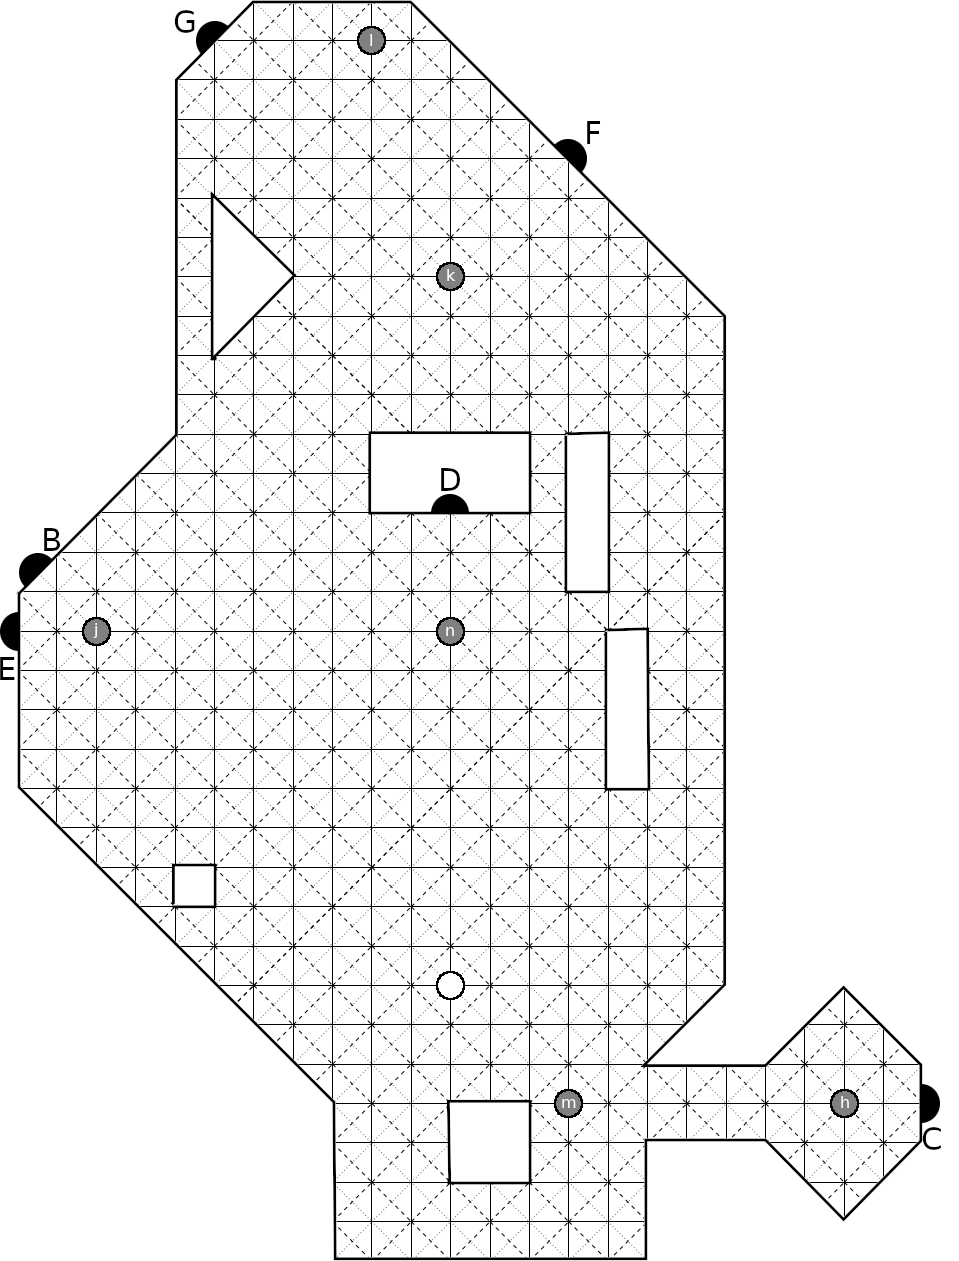
\includegraphics[scale = .6]{assets/Billiards_Puzzle3}
\end{center}

\phChapterWorksheet{Arena 4}{Balls: o, p, t, u -- Holes: A, B, C, D}

\includegraphics[width=\linewidth]{Billiards_Puzzle4}

\phChapterWorksheet{Journal Page 1}{}

{
  \Large
  \normalfont\wedn
\begin{tabular}{|ccccccc|}
  \hline
  Journal & entry & June & 28, & 3513 & & \\
  \hline
          & & & & & & \\
  \hline
          & Succesful & dig & today. & We & found & a \\
  \hline
  lot & of & pot & shards, & some & with & remarkably \\
  \hline
  intact & artwork. & Like & in & the & tomb, & there \\
  \hline
  are & scenes & of & men & with & circles & around \\
  \hline
  their & heads, & looking & to & the & sky. & We \\
  \hline
  believe & these & represent & past & kings, & deities, & or \\
  \hline
  maybe & both. & I & recall & my & advisor's & words, \\
  \hline
  ``people & are & not & pots.'' & I & should & be \\
  \hline
  careful & before & drawing & any & firm & conclusions. & On \\
  \hline
  the & other & end & of & the & site & from \\
  \hline
  the & tomb & we & found & a & burial & site. \\
  \hline
  It & was & lined & with & red & ochre, & the \\
  \hline
  bodies & were & facing & east & with & their & arms \\
  \hline
  folded. & Already & this & site & has & yielded & so \\
  \hline
  much. & If & only & the & university & understood. & They \\
  \hline
  want & to & save & money & so & badly, & but \\
  \hline
  what & is & it & for & if & not & this? \\
  \hline
\end{tabular}
}


\phChapterWorksheet{Main Puzzle 2}{The Ancient Bazaar}

The Skolem people of Mesopotamia had many myths and legends.
Dr. Jonas was particularly interested in the story of Queen Noether,
famed for her ability to barter with traders and merchants. Legend has it,
she had no trouble making some fantastic trades. Even if some
seem like bad deals, Noether could make any of the following trades,
and their opposite trades as well.

\begin{itemize}
\item One apple for one piece of meat:
  \(A\leftrightarrow M\)
\item One bottle for one magic crystal and one spice bag:
  \(B\leftrightarrow C+S\)
\item One magic crystal for two magic crystals:
  \(C\leftrightarrow 2C\)
\item One flag for one flag and one tapestry:
  \(F\leftrightarrow F+T\)
\item One loaf of bread for one apple and one piece of meat:
  \(L\leftrightarrow A+M\)
\item One piece of meat for one apple, one loaf of bread, and one piece of meat:
  \(M\leftrightarrow A+L+M\)
\item One quilt for one quilt and one tapestry:
  \(Q\leftrightarrow Q+T\)
\item One spice bag for one bottle:
  \(S\leftrightarrow B\)
\item One tapestry for one flag and one quilt:
  \(T\leftrightarrow F+Q\)
\end{itemize}

Despite this, even Noether had her limits. Sure, she could certainly exchange
two bottles for two spice bags and two magic crystals, since
\(B+B\rightarrow B+C+S\rightarrow S+S+C\rightarrow S+S+C+C\). But there's no
way she could exchange one spice bag for two bottles by using those
trades alone.

I think Dr. Jonas was investigating these limits in the November entry of her journal.
For each of the three markets, decide if each trade is possible (P) or impossible
(I). Submit your solution to ClueKeeper using the format \texttt{PIPIP} for
each market. -BF

%Of great interest to Dr. Jonas was the story of queen Noether, famed for her ability to barter with traders and merchants.
%You may have met a good haggler or two in your day, but they didn't have to deal with the strange ways of the Skolem Bazaar.
%The Skolem people had no money, instead goods were exchanged for other goods.
%Moreover, at the start of each day the shopkeepers would declare their exchange rates.
%They were notoriously stubborn and would not change these rates no matter what happened.
%
%Dr. Jonas believed that Noether was real, and wanted to learn as much about her as possible.
%Unfortunately, over time every story about Noether split into multiple versions.
%In one, Noether entered the marketplace with one bag of spice.
%\begin{itemize}
%  \item The first shopkeeper declared that 1 bag of spice is equivalent to 4 shell bracelets and 1 clay cup. (\(S \leftrightarrow 4B + C\))
%  \item The second shopkeeper declared that 1 shell bracelet is equivalent to 3 bags of spice and 3 clay cups. (\(B \leftrightarrow 3S + 3C\))
%  \item The third shopkeeper declared that 1 clay cup is equivalent to 1 bag of spice and 1 shell bracelet. (\(C \leftrightarrow S + B\))    
%\end{itemize}
%There are two versions of the story:
%\begin{enumerate}
%  \item Noether entered the bazaar with 1 bag of spice and left with exactly 7 clay cups and nothing else.
%  \item Noether entered the bazaar with 1 bag of spice and left with exactly 7 shell bracelets and nothing else.
%\end{enumerate}
%
%Dr. Jonas reasoned that the first version was possible and that the second was impossible.
%Version one could happen the following way:
%\begin{enumerate}
%  \item Go to shopkeeper 1: \(S \rightarrow 4B + C\)
%  \item Go to shopkeeper 2 and use 1 shell bracelet: \(4B + C = B + 3B + C = 3S + 3C + 3B + C = 3S + 3B + 4C\)
%  \item Go to shopkeeper 3 to get a clay cups: \(3S + 3B + 4C = 3C + 4C = 7C\)
%  \end{enumerate}
%  
%%Hint 1:
%%So why is the second version impossible? Consider the total amount of bags of spice an clay cups: \(S + C\).
%%\begin{itemize}
%%  \item The first shopkeeper does not change this amount.
%%  \item The second shopkeeper increases/decreases this amount by 6.
%%  \item The third shopkeeper does not change this amount.
%%\end{itemize}
%%Since Noether starts with \(S + C = 1\), it can only become \(1, 7, 13,\) and so on.
%%So it is impossible for her to end up with exactly \(7\) bracelets.
%%In cluekeeper, this solution would be put in as PI.
%%If there were five variants which were possible, impossible, impossible, possible, and impossible, the solution would be PIIPI.
%
%There are many more stories about Noether. If you can figure out which ones are possible and 
%which are impossible, you might be able to decipher the message hidden in Dr. Jonas' journal.


\phChapterWorksheet{Story 1}{Pomegranates, Fish, and Bread}

\begin{itemize}
\item The first shopkeeper declared that 1 pomegranate is equivalent to 1 fish. (\(P \leftrightarrow F\))
\item The second shopkeeper declared that 1 fish is equivalent to 1 pomegranate, 1 fish, and 1 loaf of bread. (\(F \leftrightarrow P + F + B\))
\item The third shopkeeper declared that 1 loaf of bread is equivalent to 1 pomegranate and 1 fish. (\(B \leftrightarrow P + F\))
\end{itemize}

Label the following versions of the story as possible or impossible.
\begin{enumerate}
\item Noether entered the bazaar with 2 pomegranates and left with 2 loaves of bread.
\item Noether entered the bazaar with 1 pomegranate and left with 3 pomegranates.
\item Noether entered the bazaar with 1 pomegranate and left with 3 poomegranates and 1 fish.
\item Noether entered the bazaar with 1 pomegranate and left with 1 loaf of bread.
\item Noether entered the bazaar with 1 pomegranate and left with 2 pomegranates.
\end{enumerate}


\phChapterWorksheet{Story 2}{Tapestries, Saddles, and Vases}

\begin{itemize}
\item The first shopkeeper declared that 1 tapestry is equivalent to 1 saddle and 1 vase. (\(T \leftrightarrow S + V\))
\item The second shopkeeper declared that 1 saddle is equivalent to 1 tapestry and 1 saddle. (\(S \leftrightarrow T + S\))
\item The third shopkeeper declared that 1 vase is equivalent to 1 tapestry and 1 vase. (\(V \leftrightarrow T + V\))
\end{itemize}

Label the following versions of the story as possible or impossible.
\begin{enumerate}
\item Noether entered the bazaar with 1 tapestry and left with 3 tapestries.
\item Noether entered the bazaar with 1 tapestry and left with 50 tapestries.
\item Noether entered the bazaar with 1 tapestry and left with 1 tapestry and 1 saddle.
\item Noether entered the bazaar with 1 tapestray and left with 1 vase.
\item Noether entered the bazaar with 2 tapestries and 1 vase and left with 1 tapestry.
\end{enumerate}



\phChapterWorksheet{Story 3}{Spice, Vases, and Magic Crystals}

Story Set-up:
\begin{itemize}
\item The first shopkeeper declared that 1 bag of spice is equivalent to 1 vase. (\(S \leftrightarrow V\))
\item The second shopkeeper declared that 1 vase is equivalent to 1 bag of spice and 1 magic crystal. (\(V \leftrightarrow S + C\))
\item The third shopkeeper declared that 1 magic crystal is worth 2 magic crystals. (\(C \leftrightarrow 2C\))
\end{itemize}

Story Versions:
\begin{enumerate}
\item Noether entered the bazaar with 1 bag of spice and left with 2 bags of spice.
\item Noether entered the bazaar with 2 bags of spice and left with 1 bag of spice and 2 vases.
\item Noether entered the bazaar with 3 bags of spice and left with 3 magic crystals.
\item Noether entered the bazaar with 1 bag of spice and left with 1 vase and 2 magic crystals.
\item Noether entered the bazaar with 4 bags of spice and left with 2 bags of spice, 2 vases, and 5 magic crystals.
\end{enumerate}


\phChapterWorksheet{Journal Page 2}{}

\begin{center}
\begin{tikzpicture}[x=0.25in,y=0.25in]
\input{assets/qrish/generate}
\begin{scope}[shift={(5,8)}] %T
  \fill[color=white] (0,0) rectangle (2,3);
%  \draw[color=cyan,thick] (0,0) rectangle (2,3);
  \fill[color=white] (0,2) rectangle (1,3);
  \fill[color=black] (1,2) rectangle (2,3);
  \fill[color=black] (0,1) rectangle (1,2);
  \fill[color=black] (1,1) rectangle (2,2);
  \fill[color=black] (0,0) rectangle (1,1);
  \fill[color=white] (1,0) rectangle (2,1);
%  \node[transform shape,color=red,anchor=west] at (2,1.5) {$\uparrow$};
\end{scope}
\begin{scope}[shift={(10,3)},rotate=180] %R
  \fill[color=white] (0,0) rectangle (2,3);
%  \draw[color=cyan,thick] (0,0) rectangle (2,3);
  \fill[color=black] (0,2) rectangle (1,3);
  \fill[color=white] (1,2) rectangle (2,3);
  \fill[color=black] (0,1) rectangle (1,2);
  \fill[color=black] (1,1) rectangle (2,2);
  \fill[color=black] (0,0) rectangle (1,1);
  \fill[color=white] (1,0) rectangle (2,1);
%  \node[transform shape,color=red,anchor=west] at (2,1.5) {$\uparrow$};
\end{scope}
\begin{scope}[shift={(1,6)}] %A
  \fill[color=white] (0,0) rectangle (2,3);
%  \draw[color=cyan,thick] (0,0) rectangle (2,3);
  \fill[color=black] (0,2) rectangle (1,3);
  \fill[color=white] (1,2) rectangle (2,3);
  \fill[color=white] (0,1) rectangle (1,2);
  \fill[color=white] (1,1) rectangle (2,2);
  \fill[color=white] (0,0) rectangle (1,1);
  \fill[color=white] (1,0) rectangle (2,1);
%  \node[transform shape,color=red,anchor=west] at (2,1.5) {$\uparrow$};
\end{scope}
\begin{scope}[shift={(10,13)},rotate=-90] %D
  \fill[color=white] (0,0) rectangle (2,3);
%  \draw[color=cyan,thick] (0,0) rectangle (2,3);
  \fill[color=black] (0,2) rectangle (1,3);
  \fill[color=black] (1,2) rectangle (2,3);
  \fill[color=white] (0,1) rectangle (1,2);
  \fill[color=black] (1,1) rectangle (2,2);
  \fill[color=white] (0,0) rectangle (1,1);
  \fill[color=white] (1,0) rectangle (2,1);
%  \node[transform shape,color=red,anchor=west] at (2,1.5) {$\uparrow$};
\end{scope}
\begin{scope}[shift={(9,4)},rotate=90] %E
  \fill[color=white] (0,0) rectangle (2,3);
%  \draw[color=cyan,thick] (0,0) rectangle (2,3);
  \fill[color=black] (0,2) rectangle (1,3);
  \fill[color=white] (1,2) rectangle (2,3);
  \fill[color=white] (0,1) rectangle (1,2);
  \fill[color=black] (1,1) rectangle (2,2);
  \fill[color=white] (0,0) rectangle (1,1);
  \fill[color=white] (1,0) rectangle (2,1);
%  \node[transform shape,color=red,anchor=west] at (2,1.5) {$\uparrow$};
\end{scope}
\end{tikzpicture}

\begin{tikzpicture}[x=0.25in,y=0.25in,rotate=90]
\fill[color=white] (0,0) rectangle (15,15);
\draw[dashed,color=gray] (0,0) rectangle (15,15);
\node at (0,0) {$+$};
\node at (15,0) {$+$};
\begin{scope}[shift={(5,8)}] %T
  \fill[color=white] (0,0) rectangle (2,3);
  \draw[color=black,thick] (0,0) rectangle (2,3);
%  \fill[color=white] (0,2) rectangle (1,3);
%  \fill[color=black] (1,2) rectangle (2,3);
%  \fill[color=black] (0,1) rectangle (1,2);
%  \fill[color=black] (1,1) rectangle (2,2);
%  \fill[color=black] (0,0) rectangle (1,1);
%  \fill[color=white] (1,0) rectangle (2,1);
  \node[transform shape,color=red,anchor=west] at (2,1.5) {$\uparrow$};
  \node[transform shape] at (1,1.5) {1};
\end{scope}
\begin{scope}[shift={(10,3)},rotate=180] %R
  \fill[color=white] (0,0) rectangle (2,3);
  \draw[color=black,thick] (0,0) rectangle (2,3);
%  \fill[color=black] (0,2) rectangle (1,3);
%  \fill[color=white] (1,2) rectangle (2,3);
%  \fill[color=black] (0,1) rectangle (1,2);
%  \fill[color=black] (1,1) rectangle (2,2);
%  \fill[color=black] (0,0) rectangle (1,1);
%  \fill[color=white] (1,0) rectangle (2,1);
  \node[transform shape,color=red,anchor=west] at (2,1.5) {$\uparrow$};
  \node[transform shape] at (1,1.5) {2};
\end{scope}
\begin{scope}[shift={(1,6)}] %A
  \fill[color=white] (0,0) rectangle (2,3);
  \draw[color=black,thick] (0,0) rectangle (2,3);
%  \fill[color=black] (0,2) rectangle (1,3);
%  \fill[color=white] (1,2) rectangle (2,3);
%  \fill[color=white] (0,1) rectangle (1,2);
%  \fill[color=white] (1,1) rectangle (2,2);
%  \fill[color=white] (0,0) rectangle (1,1);
%  \fill[color=white] (1,0) rectangle (2,1);
  \node[transform shape,color=red,anchor=west] at (2,1.5) {$\uparrow$};
  \node[transform shape] at (1,1.5) {3};
\end{scope}
\begin{scope}[shift={(10,13)},rotate=-90] %D
  \fill[color=white] (0,0) rectangle (2,3);
  \draw[color=black,thick] (0,0) rectangle (2,3);
%  \fill[color=black] (0,2) rectangle (1,3);
%  \fill[color=black] (1,2) rectangle (2,3);
%  \fill[color=white] (0,1) rectangle (1,2);
%  \fill[color=black] (1,1) rectangle (2,2);
%  \fill[color=white] (0,0) rectangle (1,1);
%  \fill[color=white] (1,0) rectangle (2,1);
  \node[transform shape,color=red,anchor=west] at (2,1.5) {$\uparrow$};
  \node[transform shape] at (1,1.5) {4};
\end{scope}
\begin{scope}[shift={(9,4)},rotate=90] %E
  \fill[color=white] (0,0) rectangle (2,3);
  \draw[color=black,thick] (0,0) rectangle (2,3);
%  \fill[color=black] (0,2) rectangle (1,3);
%  \fill[color=white] (1,2) rectangle (2,3);
%  \fill[color=white] (0,1) rectangle (1,2);
%  \fill[color=black] (1,1) rectangle (2,2);
%  \fill[color=white] (0,0) rectangle (1,1);
%  \fill[color=white] (1,0) rectangle (2,1);
  \node[transform shape,color=red,anchor=west] at (2,1.5) {$\uparrow$};
  \node[transform shape] at (1,1.5) {5};
\end{scope}
\begin{scope}[shift={(2,1)}]
  \draw[color=black,thick] (0,0) rectangle (2,3);
  \node[transform shape,color=red,anchor=west] at (2,1.5) {$\uparrow$};
\end{scope}
\begin{scope}[shift={(1,12)},rotate=-90]
  \draw[color=black,thick] (0,0) rectangle (2,3);
  \node[transform shape,color=red,anchor=west] at (2,1.5) {$\uparrow$};
\end{scope}
\begin{scope}[shift={(10,10)},rotate=180]
  \draw[color=black,thick] (0,0) rectangle (2,3);
  \node[transform shape,color=red,anchor=west] at (2,1.5) {$\uparrow$};
\end{scope}
\begin{scope}[shift={(14,5)},rotate=90]
  \draw[color=black,thick] (0,0) rectangle (2,3);
  \node[transform shape,color=red,anchor=west] at (2,1.5) {$\uparrow$};
\end{scope}
\end{tikzpicture}
\end{center}

TODOs: Cluekeeper will tell players to put the \(+\)s on the bottom
of the qr code looking thing. And obviously the 1/2/3/4/5 needs to be
replaced with some sort of extraction from the main puzzle.


\phChapterWorksheet{Main Puzzle 3}{Searching the Tombs}

The necropolis of Ramsey is a complex of underground mausoleums, buried by earth and time.
It is also where Dr. Jonas almost got fired.
After finding her first mummy, she seemed to be cursed.
Whenever she entered a new crypt, the mummy inside of it would be as far away from her team as possible.
It's not that they had a hard time finding the mummies, in fact the walls had directions on them leading straight to the sarcophagus.
Still, she had of run of impossibly bad luck.

Once the university realized how much resources Dr. Jonas was spending on her digs, they demanded she stop ``wasting'' their money.
She needed to minimize the number of rooms her team was exploring.
Using ground penetrating radar, Dr. Jonas was able to scout out possible sarcophagus locations and the passages between them.
For instance, one site looked like

\begin{center}
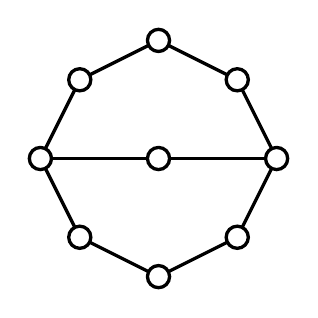
\begin{tikzpicture}[scale=0.5]
    \draw [very thick] (-3,0) -- (3,0);
    \draw [very thick] (-3,0) -- (-2,2) -- (0,3) -- (2,2) -- (3,0) -- (2,-2) -- (0,-3) -- (-2,-2) -- cycle;
    
    \filldraw [color = black, fill = white, very thick] (0,0) circle (8pt);
    \draw [color = black, fill = white, very thick] (-3,0) circle (8pt);
    \draw [color = black, fill = white, very thick] (3,0) circle (8pt);
    \draw [color = black, fill = white, very thick] (0,-3) circle (8pt);
    \draw [color = black, fill = white, very thick] (0,3) circle (8pt);
    \draw [color = black, fill = white, very thick] (2,2) circle (8pt);
    \draw [color = black, fill = white, very thick] (-2,2) circle (8pt);
    \draw [color = black, fill = white, very thick] (2,-2) circle (8pt);
    \draw [color = black, fill = white, very thick] (-2,-2) circle (8pt);
  \end{tikzpicture}
  \end{center}
  
where the circles represent rooms and the lines represent the passages connecting them.

Dr. Jonas could send 9 people out to the site and find the mummy immediately, but that's not very efficient.
Instead, she can send down just 2 people, and have the maximum number of rooms they have to explore be three 3.
Following the Univeristy accounting scheme, this has a cost of 5 as opposed to 9.
This is the best that Dr. Jonas can do.
\begin{center}
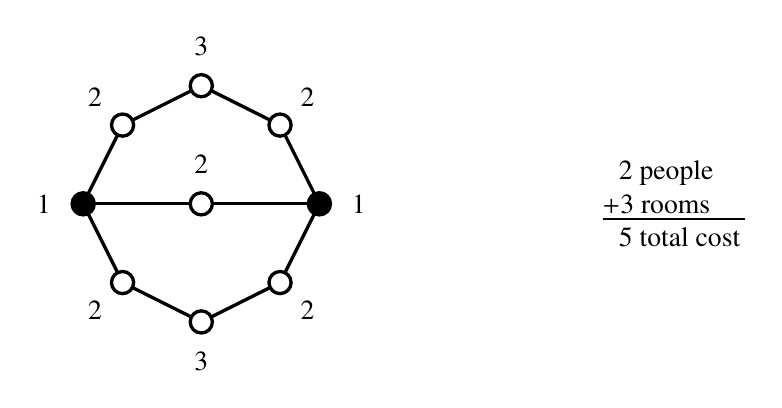
\begin{tikzpicture}[scale=0.5]
    \draw [very thick] (-3,0) -- (3,0);
    \draw [very thick] (-3,0) -- (-2,2) -- (0,3) -- (2,2) -- (3,0) -- (2,-2) -- (0,-3) -- (-2,-2) -- cycle;
    
    \draw [color = black, fill = white, very thick] (0,0) circle (8pt);
    \draw [color = black, fill = black, very thick] (-3,0) circle (8pt);
    \draw [color = black, fill = black, very thick] (3,0) circle (8pt);
    \draw [color = black, fill = white, very thick] (0,-3) circle (8pt);
    \draw [color = black, fill = white, very thick] (0,3) circle (8pt);
    \draw [color = black, fill = white, very thick] (2,2) circle (8pt);
    \draw [color = black, fill = white, very thick] (-2,2) circle (8pt);
    \draw [color = black, fill = white, very thick] (2,-2) circle (8pt);
    \draw [color = black, fill = white, very thick] (-2,-2) circle (8pt);

    \node at (0,1) {2};
    \node at (-4,0) {1};
    \node at (4,0) {1};
    \node at (0,-4) {3};
    \node at (2.7,2.7) {2};
    \node at (-2.7,2.7) {2};
    \node at (2.7,-2.7) {2};
    \node at (-2.7,-2.7) {2};
    \node at (0,4) {3};

    \node[align=left] at (12,0) {\,\, 2 people \\ \underline{+3 rooms \quad} \\ \,\, 5 total cost};
    
\end{tikzpicture}
\end{center}

There are four more site diagrams in Dr. Jonas' notes.
If you can figure out the minimum cost of exploring these crypts, B. Fraiser will be able to tell you how to deciper the next journal page.


\phChapterWorksheet{Site 1}{}

\begin{center}
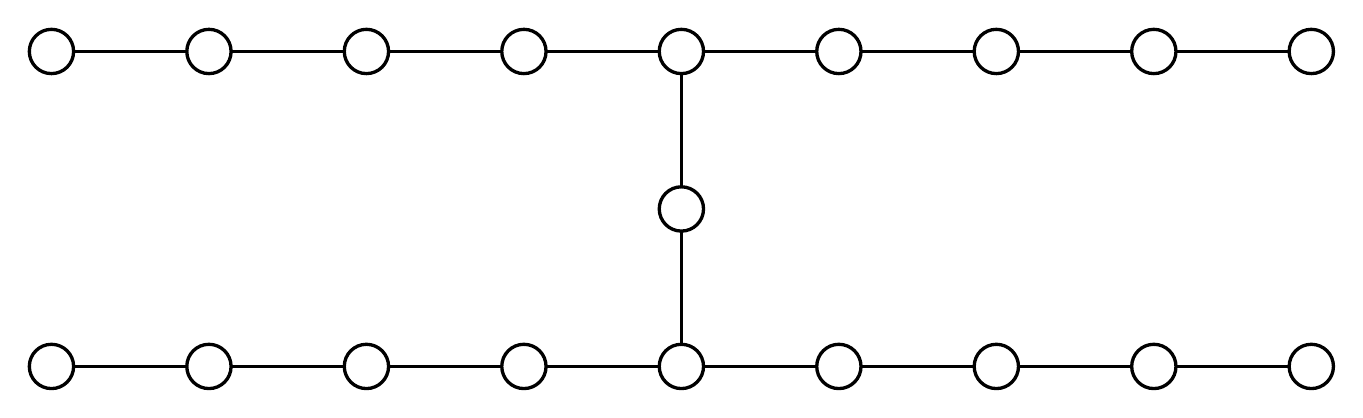
\begin{tikzpicture}
  \draw [very thick] (-8,2) -- (-6,2) -- (-4,2) -- (-2,2) -- (0,2) -- (2,2) -- (4,2) -- (6,2) -- (8,2);
  \draw [very thick] (-8,-2) -- (-6,-2) -- (-4,-2) -- (-2,-2) -- (0,-2) -- (2,-2) -- (4,-2) -- (6,-2) -- (8,-2);
  \draw [very thick] (0,2) -- (0,-2);
    
    \draw [color = black, fill = white, very thick] (-8,2) circle (8pt);
    \draw [color = black, fill = white, very thick] (-6,2) circle (8pt);
    \draw [color = black, fill = white, very thick] (-4,2) circle (8pt);
    \draw [color = black, fill = white, very thick] (-2,2) circle (8pt);
    \draw [color = black, fill = white, very thick] (0,2) circle (8pt);
    \draw [color = black, fill = white, very thick] (2,2) circle (8pt);
    \draw [color = black, fill = white, very thick] (4,2) circle (8pt);
    \draw [color = black, fill = white, very thick] (6,2) circle (8pt);
    \draw [color = black, fill = white, very thick] (8,2) circle (8pt);

    \draw [color = black, fill = white, very thick] (-8,-2) circle (8pt);
    \draw [color = black, fill = white, very thick] (-6,-2) circle (8pt);
    \draw [color = black, fill = white, very thick] (-4,-2) circle (8pt);
    \draw [color = black, fill = white, very thick] (-2,-2) circle (8pt);
    \draw [color = black, fill = white, very thick] (0,-2) circle (8pt);
    \draw [color = black, fill = white, very thick] (2,-2) circle (8pt);
    \draw [color = black, fill = white, very thick] (4,-2) circle (8pt);
    \draw [color = black, fill = white, very thick] (6,-2) circle (8pt);
    \draw [color = black, fill = white, very thick] (8,-2) circle (8pt);

    \draw [color = black, fill = white, very thick] (0,0) circle (8pt);
  \end{tikzpicture}
  \end{center}

\phChapterWorksheet{Site 2}{}

\begin{itemize}
\item The first shopkeeper declared that 1 tapestry is equivalent to 1 saddle and 1 vase. (\(T \leftrightarrow S + V\))
\item The second shopkeeper declared that 1 saddle is equivalent to 1 tapestry and 1 saddle. (\(S \leftrightarrow T + S\))
\item The third shopkeeper declared that 1 vase is equivalent to 1 tapestry and 1 vase. (\(V \leftrightarrow T + V\))
\end{itemize}

Label the following versions of the story as possible or impossible.
\begin{enumerate}
\item Noether entered the bazaar with 1 tapestry and left with 3 tapestries.
\item Noether entered the bazaar with 1 tapestry and left with 50 tapestries.
\item Noether entered the bazaar with 1 tapestry and left with 1 tapestry and 1 saddle.
\item Noether entered the bazaar with 1 tapestray and left with 1 vase.
\item Noether entered the bazaar with 2 tapestries and 1 vase and left with 1 tapestry.
\end{enumerate}



\phChapterWorksheet{Site 3}{}

\begin{center}
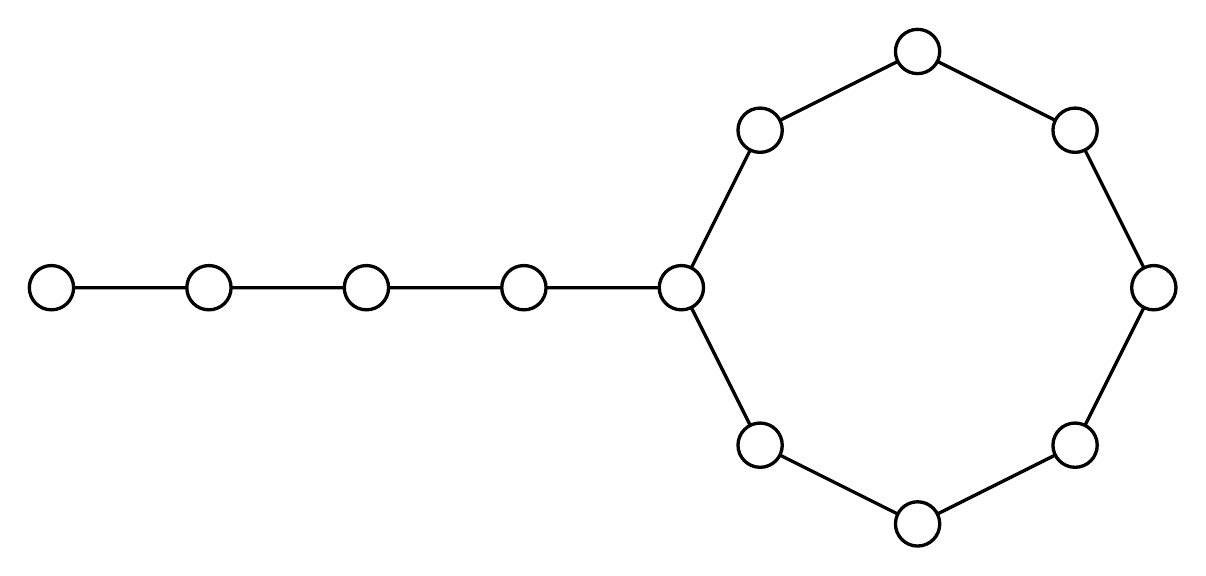
\begin{tikzpicture}
    \draw [very thick] (-11,0) -- (-9,0) -- (-7,0) -- (-5,0) -- (-3,0) -- (-2,2) -- (0,3) -- (2,2) -- (3,0) -- (2,-2) -- (0,-3) -- (-2,-2) -- (-3,0);
    
    \draw [color = black, fill = white, very thick] (-11,0) circle (8pt);
    \draw [color = black, fill = white, very thick] (-9,0) circle (8pt);
    \draw [color = black, fill = white, very thick] (-7,0) circle (8pt);
    \draw [color = black, fill = white, very thick] (-5,0) circle (8pt);
    \draw [color = black, fill = white, very thick] (-3,0) circle (8pt);
    \draw [color = black, fill = white, very thick] (3,0) circle (8pt);
    \draw [color = black, fill = white, very thick] (0,-3) circle (8pt);
    \draw [color = black, fill = white, very thick] (0,3) circle (8pt);
    \draw [color = black, fill = white, very thick] (2,2) circle (8pt);
    \draw [color = black, fill = white, very thick] (-2,2) circle (8pt);
    \draw [color = black, fill = white, very thick] (2,-2) circle (8pt);
    \draw [color = black, fill = white, very thick] (-2,-2) circle (8pt);
  \end{tikzpicture}
\end{center}
  

\phChapterWorksheet{Site 4}{}

\begin{center}
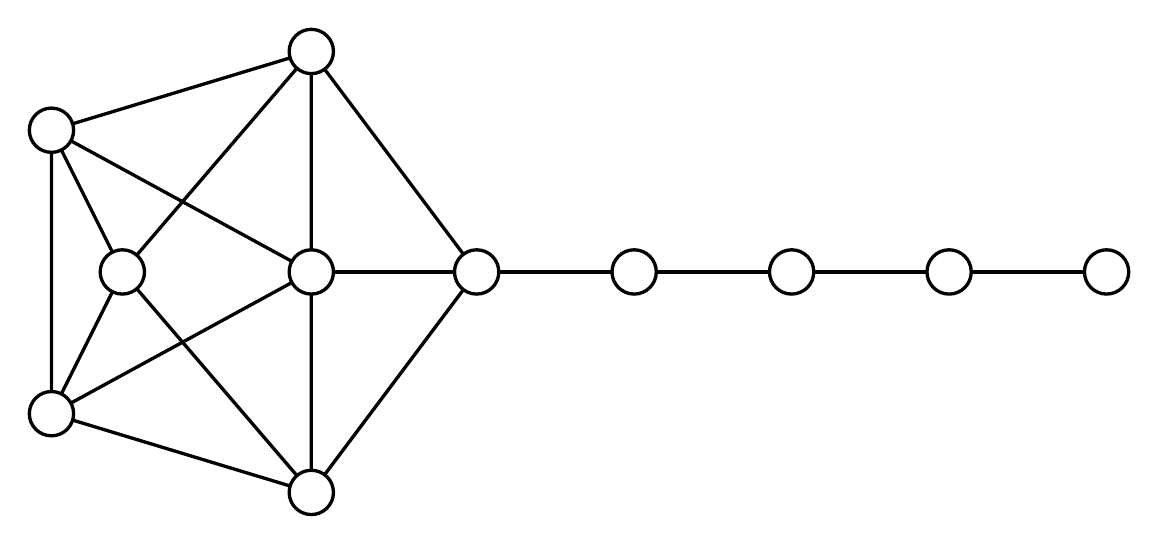
\begin{tikzpicture}
    \draw [very thick] (.9,0) -- (3,0) -- (5,0) -- (7,0) -- (9,0) -- (11,0);
    \draw [very thick] (.9, 2.8) -- (.9,-2.8) -- (-1.5,0) -- cycle;
    \draw [very thick] (-2.4, 1.8) -- (.9,0) -- (-2.4, -1.8) -- (-1.5,0) -- cycle;
    \draw [very thick] (-2.4,1.8) -- (.9,2.8) -- (3,0) -- (.9,-2.8) -- (-2.4,-1.8) -- cycle;
    
    \draw [color = black, fill = white, very thick] (11,0) circle (8pt);
    \draw [color = black, fill = white, very thick] (9,0) circle (8pt);
    \draw [color = black, fill = white, very thick] (7,0) circle (8pt);
    \draw [color = black, fill = white, very thick] (5,0) circle (8pt);
    \draw [color = black, fill = white, very thick] (-2.4,1.8) circle (8pt);
    \draw [color = black, fill = white, very thick] (.9,2.8) circle (8pt);
    \draw [color = black, fill = white, very thick] (3,0) circle (8pt);
    \draw [color = black, fill = white, very thick] (.9,-2.8) circle (8pt);
    \draw [color = black, fill = white, very thick] (-2.4,-1.8) circle (8pt);
    \draw [color = black, fill = white, very thick] (.9,0) circle (8pt);
    \draw [color = black, fill = white, very thick] (-1.5,0) circle (8pt);
  \end{tikzpicture}
  \end{center}

\phChapterWorksheet{Journal Page 3}{}

\begin{tikzpicture}
\draw[-latex] (0,0) -- (15,0);
\draw[-latex] (0,0) -- (0,15);
\foreach \x in {1,2,...,14} {
  \draw (\x,0.1) -- (\x,-0.1);
  \draw (-0.1,\x) -- (0.1,\x);
}
%\draw (2,3) -- (10,6) -- (11,11) -- (3,10) -- (2,3);
\node at (12,3) {\includegraphics[width=1in]{assets/clipart/map.png}};
\node at (4,6) {\includegraphics[width=1in]{assets/clipart/hat.png}};
\node at (8,8) {\includegraphics[width=1in]{assets/clipart/rope.png}};
\node at (3,12) {\includegraphics[width=1in]{assets/clipart/backpack.png}};
\node at (13,7) {\includegraphics[width=1in]{assets/clipart/compass.png}};
\node at (7,2) {\includegraphics[width=1in]{assets/clipart/flashlight.png}};
\end{tikzpicture}

TODO: In cluekeeper players are told to connect the coordinates
given by the previous puzzle to encircle two of the objects in
the figure. (for now, these are (2,3) (10,6) (11,11) (3,10)).
They are also told that the correct password is the combination
of two of the following words: 
BACKPACK, COMPASS, FLASHLIGHT, HAT, MAP, ROPE.


\phChapterWorksheet{Main Puzzle 4}{Ancient Gerrymandering}

One of Dr. Jonas' greatest discoveries was the Heyting people, a democratic collection of 6 tribes that lived on the Eurasian steppes.
They kept meticulous records of their elections and their rulers.
Strangely, even though the Heyting people were democratic, the voting records indicated that many of their leaders recived far less than the majority of the votes.
How could this happen?
Each tribe elected its own ruler, and then the council of 6 rulers would meet to make decisions.
To simplify the voting process, the tribes had broke their land up into provinces, each of which would cast one vote for the next ruler of that tribe.
To figure out which vote to cast, each province would take the majority vote of its people.
To cap it off, the tribe leaders were allowed to redraw the boundaries of the provinces using the following guidelines:
\begin{enumerate}
\item The number of provinces had to stay the same.
\item No province's population could exceed any others by more than 5 people.
\item All province boundary lines had to follow the grid lines provided.
\item Given two locations in the same province, you had to be able to walk between them without crossing into any other provinces.
\end{enumerate}

Altough she was unable to find records detailing the number of provinces or their boundaries, Dr. Jonas did find records detailing a three year election cycle from each of the six tribes.
The first is shown below, with possible province boundaries drawn in by Dr. Jonas.
Notice that X won all three years even though they never had the majority vote.

Tribe A
Population = 50

\begin{tabular}{c c c }

Year 1 & Year 2 & Year 3 \\
 \includegraphics[width=2in]{assets/Gerrymandering/Gerry4x4-50-1Solution.pdf} &  \includegraphics[width=2in]{assets/Gerrymandering/Gerry4x4-50-2Solution.pdf} &  \includegraphics[width=2in]{assets/Gerrymandering/Gerry4x4-50-3Solution.pdf}\\
 Total Vote Count &  Total Vote Count &  Total Vote Count\\
 X - 22 & X - 22 & X  - 22\\
 O - 28 & O - 28 & O - 28
\end{tabular}

Dr. Jonas reasoned that there were 3 provinces for tribe A.
After finding the number of provinces for the other tribes, you should be able to decode the message in Dr. Jonas' journal.


\phChapterWorksheet{Tribe B}{Population = 80}

\begin{tabular}{c c c }

Year 1 & Year 2 & Year 3 \\
 \includegraphics[width=2in]{assets/Gerrymandering/Gerry4x4-80-1.pdf} &  \includegraphics[width=2in]{assets/Gerrymandering/Gerry4x4-80-2.pdf} &  \includegraphics[width=2in]{assets/Gerrymandering/Gerry4x4-80-3.pdf}\\
 Total Vote Count &  Total Vote Count &  Total Vote Count\\
 X -  22& X - 33 & X  - 33\\
 O - 58 & O - 47 & O - 47
 \end{tabular}

\phChapterWorksheet{Tribe C}{Population = 100}

\begin{center}
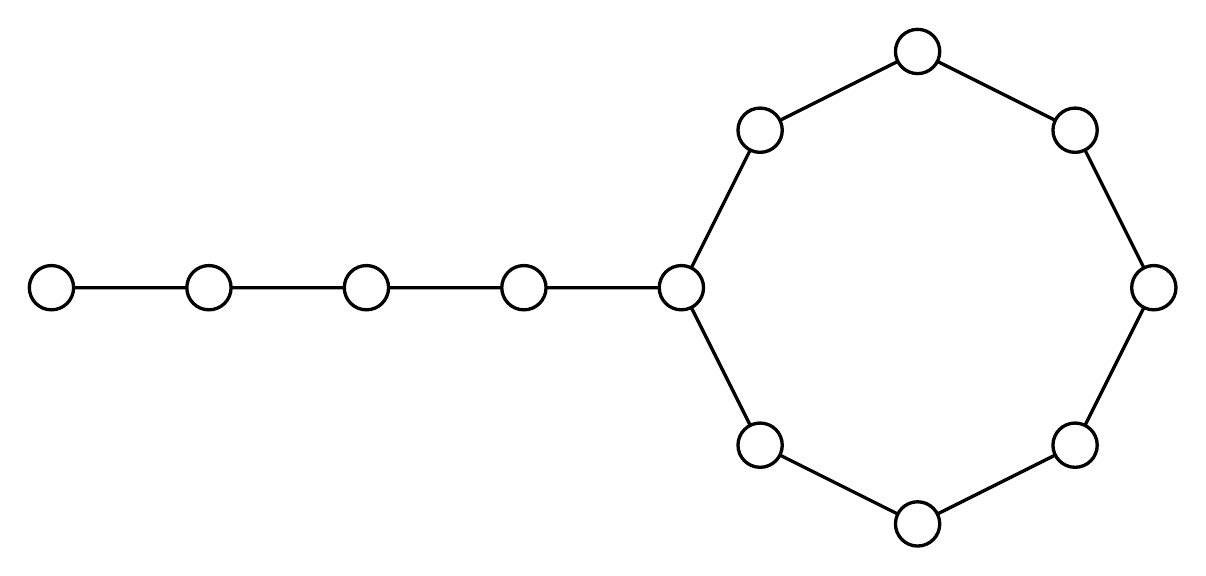
\begin{tikzpicture}
    \draw [very thick] (-11,0) -- (-9,0) -- (-7,0) -- (-5,0) -- (-3,0) -- (-2,2) -- (0,3) -- (2,2) -- (3,0) -- (2,-2) -- (0,-3) -- (-2,-2) -- (-3,0);
    
    \draw [color = black, fill = white, very thick] (-11,0) circle (8pt);
    \draw [color = black, fill = white, very thick] (-9,0) circle (8pt);
    \draw [color = black, fill = white, very thick] (-7,0) circle (8pt);
    \draw [color = black, fill = white, very thick] (-5,0) circle (8pt);
    \draw [color = black, fill = white, very thick] (-3,0) circle (8pt);
    \draw [color = black, fill = white, very thick] (3,0) circle (8pt);
    \draw [color = black, fill = white, very thick] (0,-3) circle (8pt);
    \draw [color = black, fill = white, very thick] (0,3) circle (8pt);
    \draw [color = black, fill = white, very thick] (2,2) circle (8pt);
    \draw [color = black, fill = white, very thick] (-2,2) circle (8pt);
    \draw [color = black, fill = white, very thick] (2,-2) circle (8pt);
    \draw [color = black, fill = white, very thick] (-2,-2) circle (8pt);
  \end{tikzpicture}
\end{center}
  

\phChapterWorksheet{Tribe D}{Population = 100}

\includegraphics[width=\linewidth]{Billiards_Puzzle4}

\phChapterWorksheet{Tribe E}{Population = 120}

\input{puzzles/Gerrymandering/attachment5}

\phChapterWorksheet{Tribe F}{Population = 150}

\begin{tabular}{c c c }

Year 1 & Year 2 & Year 3 \\
 \includegraphics[width=2in]{assets/Gerrymandering/Gerry5x5-150-1.pdf} &  \includegraphics[width=2in]{assets/Gerrymandering/Gerry5x5-150-2.pdf} &  \includegraphics[width=2in]{assets/Gerrymandering/Gerry5x5-150-3.pdf}\\
 Total Vote Count &  Total Vote Count &  Total Vote Count\\
 X -  50& X - 56 & X  - 58\\
 O - 100 & O - 96 & O - 92
 \end{tabular}

\phChapterWorksheet{Journal Page 4}{}

{
  \LARGE
  \normalfont\wedn
It seems that the legendary rulers of the Skolem people
were each associated with a compass direction.
Fascinating!

\renewcommand{\labelitemi}{}
\begin{itemize}
\item Oystein Apo Skolem (N)
\item Engstrom Apo Ore (NNE) % 7 O
\item Throralf Apo Thue (NE)
\item Shanok Apo Ore (ENE)
\item Trowa Apo Ore (E)
\item Mawort Apo Ore (ESE) % 5 R
\item Berkov Apo Kel (SE)
\item Knutten Apo Kel (SSE)
\item Erbach Apo Kel (S)
\item Guabis Apo Kel (SSW) % 5 I
\item Zabala Apo Dheub (SW)
\item Renfrow Apo Dheub (WSW) % 6 O
\item Frakov Apo Dheub (W)
\item Gangolli Apo Dheub (WNW) % 3 N
\item Ramkunar Apo Lewo (NW)
\item Skraba Apo Lewo (NNW)
%\item Govc Apo Preis 1686 - 1675 BCE
\end{itemize}
}


\phChapterWorksheet{Cryptic Puzzle 1}{Word Graph Thing}

  %\begin{center}
\begin{tikzpicture}[x=0.4in,y=0.4in]
% SWEATED --> SPACE
\begin{scope}[shift={(0,0)}]
\shortB\shortB\shortB
  \stStay\spaceB
\shortB\longB\longB
  \stRight{1}\spaceB
\shortB
  \stStay\spaceB
\shortB\longB
  \stStay\spaceB
\longB
  \stRight{3}\spaceB
\shortB
  \stRight{2}\spaceB
\longB\shortB\shortB
  \resetB
\end{scope}
% MATT --> GO
\begin{scope}[shift={(0,-2)}]
\longB\longB
  \stRight{1}\spaceB
\shortB\longB
  \stLeft{1}\spaceB
\longB
  \stLeft{2}\spaceB
\longB
  \resetB
\end{scope}
% URNS --> EARTH
\begin{scope}[shift={(0,-4)}]
\shortB\shortB\longB
  \stLeft{2}\stStay\spaceB
\shortB\longB\shortB
  \stStay\spaceB
\longB\shortB
  \stLeft{1}\spaceB
\shortB\shortB\shortB
  \resetB
\end{scope}
% DYE --> TITAN
\begin{scope}[shift={(0,-6)}]
\longB\shortB\shortB
  \stLeft{2}\stStay\stRight{1}\spaceB
\longB\shortB\longB\longB
  \stLeft{1}\spaceB
\shortB
  \resetB
\end{scope}
% WENCH --> ANTARES
\begin{scope}[shift={(0,-8)}]
\shortB\longB\longB
  \stLeft{1}\spaceB
\shortB
  \stStay\spaceB
\longB\shortB
  \stLeft{1}\stRight{1}\spaceB
\longB\shortB\longB\shortB
  \stStay\stRight{1}\spaceB
\shortB\shortB\shortB\shortB
  \resetB
\end{scope}
% REWIRE --> RIGEL
\begin{scope}[shift={(0,-10)}]
\shortB\longB\shortB
  \stStay\spaceB
\shortB
  \stRight{1}\spaceB
\shortB\longB\longB
  \stRight{1}\spaceB
\shortB\shortB
  \stStay\spaceB
\shortB\longB\shortB
  \stLeft{3}\spaceB
\shortB
  \resetB
\end{scope}
% CREWMEN --> CASTOR
\begin{scope}[shift={(0,-12)}]
\longB\shortB\longB\shortB
  \stStay\spaceB
\shortB\longB\shortB
  \stLeft{1}\spaceB
\shortB
  \stRight{1}\spaceB
\shortB\longB\longB
  \stLeft{1}\spaceB
\longB\longB
  \stStay\spaceB
\shortB
  \stLeft{1}\spaceB
\longB\shortB
  \resetB
\end{scope}
\end{tikzpicture}
\end{center}

%\tikzstyle{space} = [draw, circle, dotted]
%\tikzstyle{dot} = [draw, thin, circle, fill=black]
%\tikzstyle{dash} = [thick, line width=3mm, line cap=round]
%
%\newcommand{\dit}{ ++(1,0) node[dot]{} }
%\newcommand{\dah}{ ++(1,0) -- ++(2,0) }
%
%
%\newcommand{\drop}[1]{
%	\draw[->] (#1-0.5,0.5) node[space] {} -- ++(0,-2) node[space] {};
%	}
%\newcommand{\bend}[2]{
%	\draw[->] (#1-0.5,0.5) node[space] {} -- ++(0,-1) -- ++(#2,-1) node[space] {};
%	}
%
%\newcommand{\dex}[1] {++(2,-1.3) node {\sffamily\Large#1};}
%
%% SWEATED --> SPACE
%\begin{tikzpicture}[x=0.2in,y=0.2in]
%	\draw[dash] (-1,0){}
%		\dit \dit \dit %S
%		\dit \dah \dah %W
%		\dit %E
%		\dit \dah %A
%		\dah %T
%		\dit %E
%		\dah \dit \dit %D
%		\dex{2};
%	\drop{3};
%	\bend{10}{1};
%	\drop{11};
%	\drop{15};
%	\bend{18}{5};
%	\bend{19}{4};
%\end{tikzpicture}
%	
%
%\vspace{0.4in}
%
%% MATT --> GO
%\begin{tikzpicture}[x=0.2in,y=0.2in]
%	\draw[dash] (-1,0){}
%		\dah \dah %M
%		\dit \dah %A
%		\dah %T
%		\dah %T
%		\dex{2}
%		;
%	\bend{6}{1};
%	\bend{10}{-3};
%	\bend{13}{-6};
%\end{tikzpicture}
%
%\vspace{0.4in}
%
%% URNS --> EARTH
%\begin{tikzpicture}[x=0.2in,y=0.2in]
%	\draw[dash] (-1,0){}
%		\dit \dit \dah %U
%		\dit \dah \dit %R
%		\dah \dit %N
%		\dit \dit \dit %S
%		\dex{3}
%		;
%	\bend{5}{-4};
%	\drop{5};
%	\drop{10};
%	\bend{14}{-1};
%\end{tikzpicture}
%
%\vspace{0.4in}
%
%% DYE --> TITAN
%\begin{tikzpicture}[x=0.2in,y=0.2in]
%	\draw[dash] (-1,0){}
%		\dah \dit \dit %D
%		\dah \dit \dah \dah %Y
%		\dit %E
%		\dex{3}
%		;
%	\bend{5}{-2};
%	\drop{5};
%	\bend{5}{3};
%	\bend{15}{-3};
%\end{tikzpicture}
%
%\vspace{0.4in}
%
%% WENCH --> ANTARES
%\begin{tikzpicture}[x=0.2in,y=0.2in]
%	\draw[dash] (-1,0){}
%		\dit \dah \dah %W
%		\dit %E
%		\dah \dit %N
%		\dah \dit \dah \dit %C
%		\dit \dit \dit \dit %H
%		\dex{1}
%		;
%	\bend{7}{-3};
%	\drop{8};
%	\bend{12}{-1};
%	\bend{12}{3};
%	\drop{20};
%	\bend{20}{1};
%\end{tikzpicture}
%
%\vspace{0.4in}
%
%% REWIRE --> RIGEL
%\begin{tikzpicture}[x=0.2in,y=0.2in]
%	\draw[dash] (-1,0){}
%		\dit \dah \dit %R
%		\dit %E
%		\dit \dah \dah %W
%		\dit \dit %I
%		\dit \dah \dit %R
%		\dit %E
%		\dex{5}
%		;
%	\drop{5};
%	\bend{6}{1};
%	\bend{13}{1};
%	\drop{15};
%	\bend{20}{-5};
%\end{tikzpicture}
%
%\vspace{0.4in}
%
%% CREWMEN --> CASTOR
%\begin{tikzpicture}[x=0.2in,y=0.2in]
%	\draw[dash] (-1,0){}
%		\dah \dit \dah \dit %C
%		\dit \dah \dit %R
%		\dit %E
%		\dit \dah \dah %W
%		\dah \dah %M
%		\dit %E
%		\dah \dit %N
%		\dex{3}
%		;
%	\drop{8};
%	\bend{13}{-1};
%	\bend{14}{1};
%	\bend{21}{-3};
%	\drop{27};
%	\bend{28}{-1};
%\end{tikzpicture}


\phChapterWorksheet{Cryptic Puzzle 2}{Linguistic Drift}

Language changes over time, sometimes in strange ways.
In this journal page Dr. Jonas was considering the changes in an ancient script over a period of 450 years and then 600 years.
It looks like she hid a message in the unfinished 600 year group.

Here is a brief crash course in linguistics: you can expect a major change to occur every 150 years.
Keep an eye out for changes in boundaries, contractions, and expansions.
Good luck!


\phChapterWorksheet{Cryptic Puzzle 3}{Simon Says}

Shortly before she disappeared, Dr. Jonas was obsessed with studying the designs
found on the dice used by the ancient Heyting people. It seems that between
one and seven pips would be handcarved into the sides of a cube. While the position 
of the pips wouldn't affect the value of the roll (two pips always has a value of \(2\), 
no matter how they are arranged), some pip designs were considered
sacred, while the rest were known as profane.

I don't know the rules for what makes a pip design sacred or not, but I've attached
some examples from Dr. Jonas's notes. Maybe they'll be of some use in understanding
one of her journal entires. -BF

\begin{center}
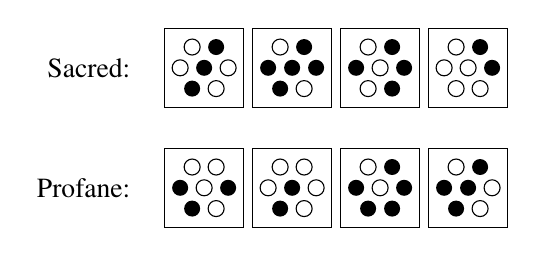
\begin{tikzpicture}[x=0.04in,y=0.04in]
\begin{scope}[shift={(0,0)}]
\node[anchor=east] at (-180:8) {Sacred:};
\draw (-45:7) rectangle (135:7);
\fill (0:0) circle (1);
\draw (0:3) circle (1);
\fill (60:3) circle (1);
\draw (120:3) circle (1);
\draw (180:3) circle (1);
\fill (-120:3) circle (1);
\draw (-60:3) circle (1);
\end{scope}
\begin{scope}[shift={(11,0)}]
\draw (-45:7) rectangle (135:7);
\fill (0:0) circle (1);
\fill (0:3) circle (1);
\fill (60:3) circle (1);
\draw (120:3) circle (1);
\fill (180:3) circle (1);
\fill (-120:3) circle (1);
\draw (-60:3) circle (1);
\end{scope}
\begin{scope}[shift={(22,0)}]
\draw (-45:7) rectangle (135:7);
\draw (0:0) circle (1);
\fill (0:3) circle (1);
\fill (60:3) circle (1);
\draw (120:3) circle (1);
\fill (180:3) circle (1);
\draw (-120:3) circle (1);
\fill (-60:3) circle (1);
\end{scope}
\begin{scope}[shift={(33,0)}]
\draw (-45:7) rectangle (135:7);
\draw (0:0) circle (1);
\fill (0:3) circle (1);
\fill (60:3) circle (1);
\draw (120:3) circle (1);
\draw (180:3) circle (1);
\draw (-120:3) circle (1);
\draw (-60:3) circle (1);
\end{scope}
\begin{scope}[shift={(0,-15)}]
\node[anchor=east] at (-180:8) {Profane:};
\draw (-45:7) rectangle (135:7);
\draw (0:0) circle (1);
\fill (0:3) circle (1);
\draw (60:3) circle (1);
\draw (120:3) circle (1);
\fill (180:3) circle (1);
\fill (-120:3) circle (1);
\draw (-60:3) circle (1);
\end{scope}
\begin{scope}[shift={(11,-15)}]
\draw (-45:7) rectangle (135:7);
\fill (0:0) circle (1);
\draw (0:3) circle (1);
\draw (60:3) circle (1);
\draw (120:3) circle (1);
\draw (180:3) circle (1);
\fill (-120:3) circle (1);
\draw (-60:3) circle (1);
\end{scope}
\begin{scope}[shift={(22,-15)}]
\draw (-45:7) rectangle (135:7);
\draw (0:0) circle (1);
\fill (0:3) circle (1);
\fill (60:3) circle (1);
\draw (120:3) circle (1);
\fill (180:3) circle (1);
\fill (-120:3) circle (1);
\fill (-60:3) circle (1);
\end{scope}
\begin{scope}[shift={(33,-15)}]
\draw (-45:7) rectangle (135:7);
\fill (0:0) circle (1);
\draw (0:3) circle (1);
\fill (60:3) circle (1);
\draw (120:3) circle (1);
\fill (180:3) circle (1);
\fill (-120:3) circle (1);
\draw (-60:3) circle (1);
\end{scope}
\end{tikzpicture}
\end{center}



%This mostly ordinary journal has strange doodles at the start of each line.
%In fact these are pictures of early dice from the Heyting people, or at least some of them are.
%Dr. Jonas was a Heyting expert, so there is no way she drew incorrect dice on accident.
%Both of the dates at the beginning look wrong as well.
%Dr. Jonas must have put them there for some other purpose.


\phChapterWorksheet{Cryptic Puzzle 4}{Accounting}

  %\begin{center}
\includegraphics[width=\linewidth]{assets/star-wars-resized.pdf}
\end{center}

%For %3
%a %1
%time %4
%I %1
%tried %5
%carefully %9
%to %2
%detail %6
%biographies %B, not 5
%via %3
%large %5
%crawling %8
%textboxes. %9
%
%Lamentably, %L, not 7
%composing %9
%all %3
%of %2
%the %3
%anecdotes %A, not 8
%when %4
%curbed %6
%by %2
%finite %6
%room, %4
%the %3
%current %C, not 3
%strategy %8
%now %3
%is %2
%cruelly %7
%killing %K, not 9
%sound %5
%handwriting. %H, not 0
%
%To %2
%sidestep %8
%probable %8
%oversights %O, not 4
%I %1
%intensely %9
%loathe, %L, not 7
%I %1
%entreat %E, not 6
%humankind, %9
%ban %3
%laughable %9
%cuneiform! %9


\phChapterWorksheet{Bonus Puzzle}{Azul Puzzle}

  %\includegraphics[width=\linewidth]{assets/wormhole-alpha}


\phChapterWorksheet{Meta Puzzle}{Alien Conversation}

  %\begin{center}
\begin{tikzpicture}[x=0.4in,y=0.4in]
% SWEATED --> SPACE
\begin{scope}[shift={(0,0)}]
\shortB\shortB\shortB
  \stStay\spaceB
\shortB\longB\longB
  \stRight{1}\spaceB
\shortB
  \stStay\spaceB
\shortB\longB
  \stStay\spaceB
\longB
  \stRight{3}\spaceB
\shortB
  \stRight{2}\spaceB
\longB\shortB\shortB
  \resetB
\end{scope}
% MATT --> GO
\begin{scope}[shift={(0,-2)}]
\longB\longB
  \stRight{1}\spaceB
\shortB\longB
  \stLeft{1}\spaceB
\longB
  \stLeft{2}\spaceB
\longB
  \resetB
\end{scope}
% URNS --> EARTH
\begin{scope}[shift={(0,-4)}]
\shortB\shortB\longB
  \stLeft{2}\stStay\spaceB
\shortB\longB\shortB
  \stStay\spaceB
\longB\shortB
  \stLeft{1}\spaceB
\shortB\shortB\shortB
  \resetB
\end{scope}
% DYE --> TITAN
\begin{scope}[shift={(0,-6)}]
\longB\shortB\shortB
  \stLeft{2}\stStay\stRight{1}\spaceB
\longB\shortB\longB\longB
  \stLeft{1}\spaceB
\shortB
  \resetB
\end{scope}
% WENCH --> ANTARES
\begin{scope}[shift={(0,-8)}]
\shortB\longB\longB
  \stLeft{1}\spaceB
\shortB
  \stStay\spaceB
\longB\shortB
  \stLeft{1}\stRight{1}\spaceB
\longB\shortB\longB\shortB
  \stStay\stRight{1}\spaceB
\shortB\shortB\shortB\shortB
  \resetB
\end{scope}
% REWIRE --> RIGEL
\begin{scope}[shift={(0,-10)}]
\shortB\longB\shortB
  \stStay\spaceB
\shortB
  \stRight{1}\spaceB
\shortB\longB\longB
  \stRight{1}\spaceB
\shortB\shortB
  \stStay\spaceB
\shortB\longB\shortB
  \stLeft{3}\spaceB
\shortB
  \resetB
\end{scope}
% CREWMEN --> CASTOR
\begin{scope}[shift={(0,-12)}]
\longB\shortB\longB\shortB
  \stStay\spaceB
\shortB\longB\shortB
  \stLeft{1}\spaceB
\shortB
  \stRight{1}\spaceB
\shortB\longB\longB
  \stLeft{1}\spaceB
\longB\longB
  \stStay\spaceB
\shortB
  \stLeft{1}\spaceB
\longB\shortB
  \resetB
\end{scope}
\end{tikzpicture}
\end{center}

%\tikzstyle{space} = [draw, circle, dotted]
%\tikzstyle{dot} = [draw, thin, circle, fill=black]
%\tikzstyle{dash} = [thick, line width=3mm, line cap=round]
%
%\newcommand{\dit}{ ++(1,0) node[dot]{} }
%\newcommand{\dah}{ ++(1,0) -- ++(2,0) }
%
%
%\newcommand{\drop}[1]{
%	\draw[->] (#1-0.5,0.5) node[space] {} -- ++(0,-2) node[space] {};
%	}
%\newcommand{\bend}[2]{
%	\draw[->] (#1-0.5,0.5) node[space] {} -- ++(0,-1) -- ++(#2,-1) node[space] {};
%	}
%
%\newcommand{\dex}[1] {++(2,-1.3) node {\sffamily\Large#1};}
%
%% SWEATED --> SPACE
%\begin{tikzpicture}[x=0.2in,y=0.2in]
%	\draw[dash] (-1,0){}
%		\dit \dit \dit %S
%		\dit \dah \dah %W
%		\dit %E
%		\dit \dah %A
%		\dah %T
%		\dit %E
%		\dah \dit \dit %D
%		\dex{2};
%	\drop{3};
%	\bend{10}{1};
%	\drop{11};
%	\drop{15};
%	\bend{18}{5};
%	\bend{19}{4};
%\end{tikzpicture}
%	
%
%\vspace{0.4in}
%
%% MATT --> GO
%\begin{tikzpicture}[x=0.2in,y=0.2in]
%	\draw[dash] (-1,0){}
%		\dah \dah %M
%		\dit \dah %A
%		\dah %T
%		\dah %T
%		\dex{2}
%		;
%	\bend{6}{1};
%	\bend{10}{-3};
%	\bend{13}{-6};
%\end{tikzpicture}
%
%\vspace{0.4in}
%
%% URNS --> EARTH
%\begin{tikzpicture}[x=0.2in,y=0.2in]
%	\draw[dash] (-1,0){}
%		\dit \dit \dah %U
%		\dit \dah \dit %R
%		\dah \dit %N
%		\dit \dit \dit %S
%		\dex{3}
%		;
%	\bend{5}{-4};
%	\drop{5};
%	\drop{10};
%	\bend{14}{-1};
%\end{tikzpicture}
%
%\vspace{0.4in}
%
%% DYE --> TITAN
%\begin{tikzpicture}[x=0.2in,y=0.2in]
%	\draw[dash] (-1,0){}
%		\dah \dit \dit %D
%		\dah \dit \dah \dah %Y
%		\dit %E
%		\dex{3}
%		;
%	\bend{5}{-2};
%	\drop{5};
%	\bend{5}{3};
%	\bend{15}{-3};
%\end{tikzpicture}
%
%\vspace{0.4in}
%
%% WENCH --> ANTARES
%\begin{tikzpicture}[x=0.2in,y=0.2in]
%	\draw[dash] (-1,0){}
%		\dit \dah \dah %W
%		\dit %E
%		\dah \dit %N
%		\dah \dit \dah \dit %C
%		\dit \dit \dit \dit %H
%		\dex{1}
%		;
%	\bend{7}{-3};
%	\drop{8};
%	\bend{12}{-1};
%	\bend{12}{3};
%	\drop{20};
%	\bend{20}{1};
%\end{tikzpicture}
%
%\vspace{0.4in}
%
%% REWIRE --> RIGEL
%\begin{tikzpicture}[x=0.2in,y=0.2in]
%	\draw[dash] (-1,0){}
%		\dit \dah \dit %R
%		\dit %E
%		\dit \dah \dah %W
%		\dit \dit %I
%		\dit \dah \dit %R
%		\dit %E
%		\dex{5}
%		;
%	\drop{5};
%	\bend{6}{1};
%	\bend{13}{1};
%	\drop{15};
%	\bend{20}{-5};
%\end{tikzpicture}
%
%\vspace{0.4in}
%
%% CREWMEN --> CASTOR
%\begin{tikzpicture}[x=0.2in,y=0.2in]
%	\draw[dash] (-1,0){}
%		\dah \dit \dah \dit %C
%		\dit \dah \dit %R
%		\dit %E
%		\dit \dah \dah %W
%		\dah \dah %M
%		\dit %E
%		\dah \dit %N
%		\dex{3}
%		;
%	\drop{8};
%	\bend{13}{-1};
%	\bend{14}{1};
%	\bend{21}{-3};
%	\drop{27};
%	\bend{28}{-1};
%\end{tikzpicture}



\end{document}
